\documentclass[11pt,a4paper]{article}

% ---------- packages ----------
\usepackage[utf8]{inputenc}
\usepackage[T1]{fontenc}
\usepackage[margin=2.4cm]{geometry}
\usepackage{graphicx}
\usepackage{booktabs}
\usepackage{amsmath,amssymb}
\usepackage{siunitx}
\usepackage[hidelinks]{hyperref}
\usepackage{caption}
\usepackage{subcaption}
\usepackage{authblk}
\usepackage{titlesec}

% ---------- light formatting ----------
\titleformat{\section}{\large\bfseries}{\thesection}{0.6em}{}
\titleformat{\subsection}{\normalsize\bfseries}{\thesubsection}{0.6em}{}
\setlength{\parskip}{0.35em}
\setlength{\parindent}{1.1em}
\captionsetup{font=small,labelfont=bf}
\sisetup{group-separator={,},group-minimum-digits=4}

% ---------- title ----------
\title{\vspace{-1.2cm}\bfseries Data-Driven Phenotyping of Sleep Signals via
Clustering: Unsupervised, Semi-Supervised and Deep Representation Approaches on
Multi-Modal Polysomnography in the MESA Cohort}

\author[1]{Naman Kansal}
\author[1]{\normalsize Supervisors: Dr Jie Yang, Professor Wei Chen}
\affil[1]{\normalsize School of Biomedical Engineering, The University of Sydney}
\date{\normalsize SCDL3991 Science Dalyell Individual Research Project, June 2026}

\begin{document}
\maketitle

\begin{abstract}
\noindent\small
The American Academy of Sleep Medicine (AASM) partitions sleep into five stages
scored by visual inspection of polysomnography (PSG). Whether these five stages
emerge naturally from the physiological signals themselves, without expert labels,
is an open question of theoretical and clinical importance: a positive answer
would provide data-driven support for the five-stage paradigm and a route to
staging where labels are scarce. We investigate this through unsupervised
clustering of PSG from 100 subjects (\num{127401} thirty-second epochs) of the
Multi-Ethnic Study of Atherosclerosis (MESA) Sleep cohort. Starting from a
heart-rate-variability baseline that recovered essentially no stage structure
(adjusted Rand index, ARI, $\approx 0.025$), we show that the representation,
rather than the clustering algorithm, is the dominant factor. A 39-dimensional set
of spectral electroencephalography (EEG) features combined with temporal context
and density-based clustering recovered the five stages at $\text{ARI}=0.28$ and
\SI{61.7}{\percent} accuracy (Cohen's $\kappa=0.40$), far above a calibrated random
baseline (ARI $\approx 0$). Gaussian mixture and density clustering outperformed
$k$-means because sleep stages form unequal, non-spherical groups, and a
per-subject hidden Markov model best recovered the minority stages (balanced
accuracy \SI{48.1}{\percent}). A small labelling budget proved highly
cost-effective: semi-supervised label propagation with \SI{10}{\percent} of labels
reached \SI{66.3}{\percent} accuracy on unseen subjects under leakage-free
cross-validation. Finally, three families of deep representation learning and
consensus clustering all underperformed the classical pipeline at this dataset
scale, an informative negative result. Together these findings give qualified,
data-driven support for the five-stage paradigm and identify feature representation
and temporal structure as the highest-leverage ingredients for unsupervised sleep
staging.
\end{abstract}

% =====================================================================
\section{Introduction}
% =====================================================================
Sleep staging is the foundation of clinical sleep medicine, underpinning the
assessment of sleep architecture and the diagnosis of disorders such as insomnia,
narcolepsy and sleep-disordered breathing. The AASM scoring manual, derived from
the earlier Rechtschaffen and Kales rules through expert consensus, divides sleep
into five stages: Wake (W), N1, N2, N3 and rapid eye movement (REM)~\cite{aasm}.
Scoring is performed by trained technicians who visually inspect the
electroencephalogram (EEG), electrooculogram (EOG) and electromyogram (EMG) in
30-second epochs.

Despite its central role, the framework has two well-documented limitations.
First, the choice of exactly five stages rests largely on historical consensus
rather than direct empirical evidence that physiology organises into five discrete
states; the merger of the former stages 3 and 4 into a single N3 was itself driven
by the absence of evidence distinguishing them~\cite{ma2026}. Second, visual
scoring shows limited inter-rater agreement, particularly at stage transitions and
for the minority stages N1 and N3, because human experts differ in their
perceptual sensitivity to transient neural patterns~\cite{ma2026}. These
limitations motivate a data-driven question that frames the present project:
\emph{if PSG epochs are clustered without any access to expert labels, do the
resulting groups correspond to the five AASM stages?}

This question was recently addressed by Ma et al.~\cite{ma2026}, who applied fuzzy
subspace clustering to an extensive set of EEG, EOG and EMG features from the MNC
and HMC databases and found that five clusters optimally described the data,
broadly aligning with the AASM stages. Their study substantiates the five-stage
paradigm but also argues that supervised staging models, which reach roughly
\SI{80}{\percent} agreement, are fundamentally ``expert imitators'' that inherit
the subjectivity of the labels they learn from. Unsupervised analysis is therefore
not merely a low-resource alternative to supervised staging but a way to probe the
neurophysiological basis of the staging system itself.

Ma et al.\ are not the first to approach staging without labels. Earlier
unsupervised and mixture-model studies established that clustering of EEG spectral
features can separate the broad NREM--REM--Wake structure but struggles to resolve
the lighter stages, foreshadowing the per-stage gradient we observe~\cite{guenoune}.
A separate body of work has probed how far cardiac autonomic signals alone can go:
HRV-based staging recovers sleep/wake and, less reliably, REM/NREM contrasts, but
consistently fails at the full five-stage resolution because autonomic tone is only
loosely coupled to cortical state~\cite{boudreau}. This established HRV ceiling is
precisely what our own ECG baseline reproduces, and it is the empirical basis for
our shift to EEG-centred representations. A complementary lesson in rigour comes
from Levy et al.~\cite{levy2023}, whose deep model for obstructive sleep apnea,
trained on \num{12923} recordings across six databases, reported performance with
bootstrap confidence intervals, the intraclass correlation coefficient,
macro-averaged $F_1$, per-cohort confusion matrices and significance tests. We adopt
the same standards of calibration and uncertainty reporting here.

This project investigates unsupervised recovery of the AASM stages from MESA
polysomnography, with two supporting questions about how that recovery can be
strengthened. The work evolved through a deliberate sequence. An initial baseline
using heart-rate-variability (HRV) features from the electrocardiogram (ECG)
recovered almost no stage structure (external agreement near zero;
Figure~\ref{fig:baseline}), confirming the established view that autonomic signals
alone are insufficient for fine-grained staging~\cite{ma2026} and motivating a
shift to EEG-centred, multi-modal and richer feature representations. That
progression, from an impoverished representation to one that recovers the stages,
is the spine of this report.

\subsection{Aims}
\begin{enumerate}\itemsep0.1em
\item To determine how well fully unsupervised clustering of MESA physiology
recovers the five AASM stages, and to identify which feature representation and
clustering algorithm maximise external agreement (the primary aim).
\item To quantify the additional gain from incorporating temporal structure and a
small labelling budget through semi-supervised learning.
\item To test rigorously whether modern deep representation learning improves on
classical engineered features at this dataset scale, reporting negative results
with the same care as positive ones.
\end{enumerate}

% =====================================================================
\section{Methods}
% =====================================================================
\subsection{Dataset}
We used the MESA Sleep Study, an ancillary study of the Multi-Ethnic Study of
Atherosclerosis comprising overnight PSG for 2{,}056 subjects, distributed via the
National Sleep Research Resource (NSRR)~\cite{zhang2018,chen2015}. Each recording
provides EEG, EOG, EMG, ECG (\SI{256}{\hertz}), oxygen saturation
(SpO\textsubscript{2}, \SI{1}{\hertz}) and thoracic/abdominal respiratory effort
(\SI{32}{\hertz}), with expert AASM stage annotations on a 30-second epoch grid. A
fixed random subset of 100 subjects (seed 42) was processed, yielding \num{127401}
labelled epochs. The stage distribution is strongly imbalanced, with N2 and Wake
dominant and N1 and N3 in the minority, a property any clustering method must
contend with because most algorithms implicitly favour balanced clusters.

\subsection{Preprocessing}
The pipeline follows the structure of Ma et al.~\cite{ma2026} with deliberate
adaptations for the MESA cohort. Signals were loaded from EDF, band-pass filtered
(\SIrange{0.3}{35}{\hertz} for EEG), and a \SI{60}{\hertz} notch filter was applied
to remove United States power-line interference (Ma et al.\ used \SI{50}{\hertz}
for their European and Chinese data). Recordings were segmented into 30-second
non-overlapping epochs aligned with the AASM annotation grid, and per-epoch feature
vectors were extracted and $z$-score normalised, with missing values
median-imputed. All preprocessing code is available in the project repository for
reproducibility.

\subsection{Feature representations}
Three representations were compared, reflecting the project's progression.
\emph{(i) HRV baseline:} seven time, frequency and nonlinear HRV features from the
ECG, the established standard for autonomic analysis. \emph{(ii) Band-power EEG:}
15 features (five canonical bands $\times$ three EEG channels). \emph{(iii) Rich
EEG:} 39 features (13 per channel) comprising five relative band powers, spectral
entropy, spectral edge frequency, spectral centroid, the three Hjorth parameters
(activity, mobility, complexity), the delta/beta ratio and the zero-crossing rate.
The rich set captures spectral shape and signal complexity that band powers
discard, and was motivated by supervisor feedback that the feature space, rather
than the algorithm, sets the ceiling on achievable performance. We additionally
evaluated multi-modal fusion by concatenating EMG, SpO\textsubscript{2} and
respiratory features with the EEG representation.

\subsection{Temporal context}
Because sleep is temporally smooth, with adjacent epochs very likely to share a
stage, each epoch's feature vector was augmented with the mean of its neighbours in
a five-epoch window, computed within each recording so as not to cross subject
boundaries. A five-epoch (2.5-minute) window was chosen as a balance between
capturing local stage continuity and avoiding the over-smoothing of genuine
transitions that wider windows cause; in preliminary tests it gave the most stable
gain, and windows beyond roughly seven epochs began to blur stage boundaries. This
encodes local temporal proximity without using any labels and doubles the feature
dimension.

\subsection{Clustering and dimensionality reduction}
We evaluated $k$-means, Gaussian mixture models (GMM; full, diagonal and spherical
covariances), agglomerative clustering, DBSCAN and HDBSCAN. Principal component
analysis (PCA) and uniform manifold approximation and projection (UMAP) were
compared for dimensionality reduction. The number of clusters was fixed to five to
test correspondence with the AASM stages, following Ma et al.~\cite{ma2026}. For
DBSCAN, the neighbourhood radius $\varepsilon$ was examined using the $k$-distance
graph (Figure~\ref{fig:kdist}) rather than tuned against labels. The $k$-distance
elbow for the rich-feature space lies well above the values that proved useful for
five-cluster recovery; we report results at $\varepsilon=2.0$, a value on the lower,
denser part of the curve that yielded the most stable five-way partition. We note
this as a limitation of unsupervised radius selection: the global elbow heuristic
does not by itself identify the radius best suited to recovering the specific
number of clusters of interest, and our choice, while not tuned against labels, was
guided by clustering stability rather than the elbow alone. A per-subject Gaussian hidden Markov
model (HMM; five states, full covariance, fitted by Baum--Welch) modelled
stage-transition dynamics explicitly. Emission means were initialised from a
$k$-means partition of each subject's epochs, the transition matrix was initialised
near-diagonal to reflect the high self-transition probability of sleep stages, and
fitting used up to 50 expectation--maximisation iterations with a fixed random seed
for reproducibility.

\subsection{Semi-supervised and supervised references}
To quantify the value of a small labelling budget, label spreading
($k$-nearest-neighbour graph propagation, $k=20$) and self-training (a random
forest iteratively augmented with its own confident predictions) were evaluated
with 5--\SI{20}{\percent} of labels, scored only on held-out unlabelled epochs. A
fully supervised random forest (\SI{100}{\percent} labels) provides an upper-bound
reference; it is not proposed as a staging method.

\subsection{Evaluation}
Cluster-to-label correspondence was established by optimal (Hungarian) assignment.
We report ARI and normalised mutual information (NMI), which are
permutation-invariant, alongside accuracy, balanced accuracy, Cohen's $\kappa$ and
macro-$F_1$. Following Levy et al.~\cite{levy2023}, all results are calibrated
against a random-assignment baseline, and the semi-supervised analyses use
\emph{subject-level} five-fold cross-validation (no subject in both training and
evaluation), reported as mean $\pm$ standard deviation across folds.

\begin{figure}[t]
\centering
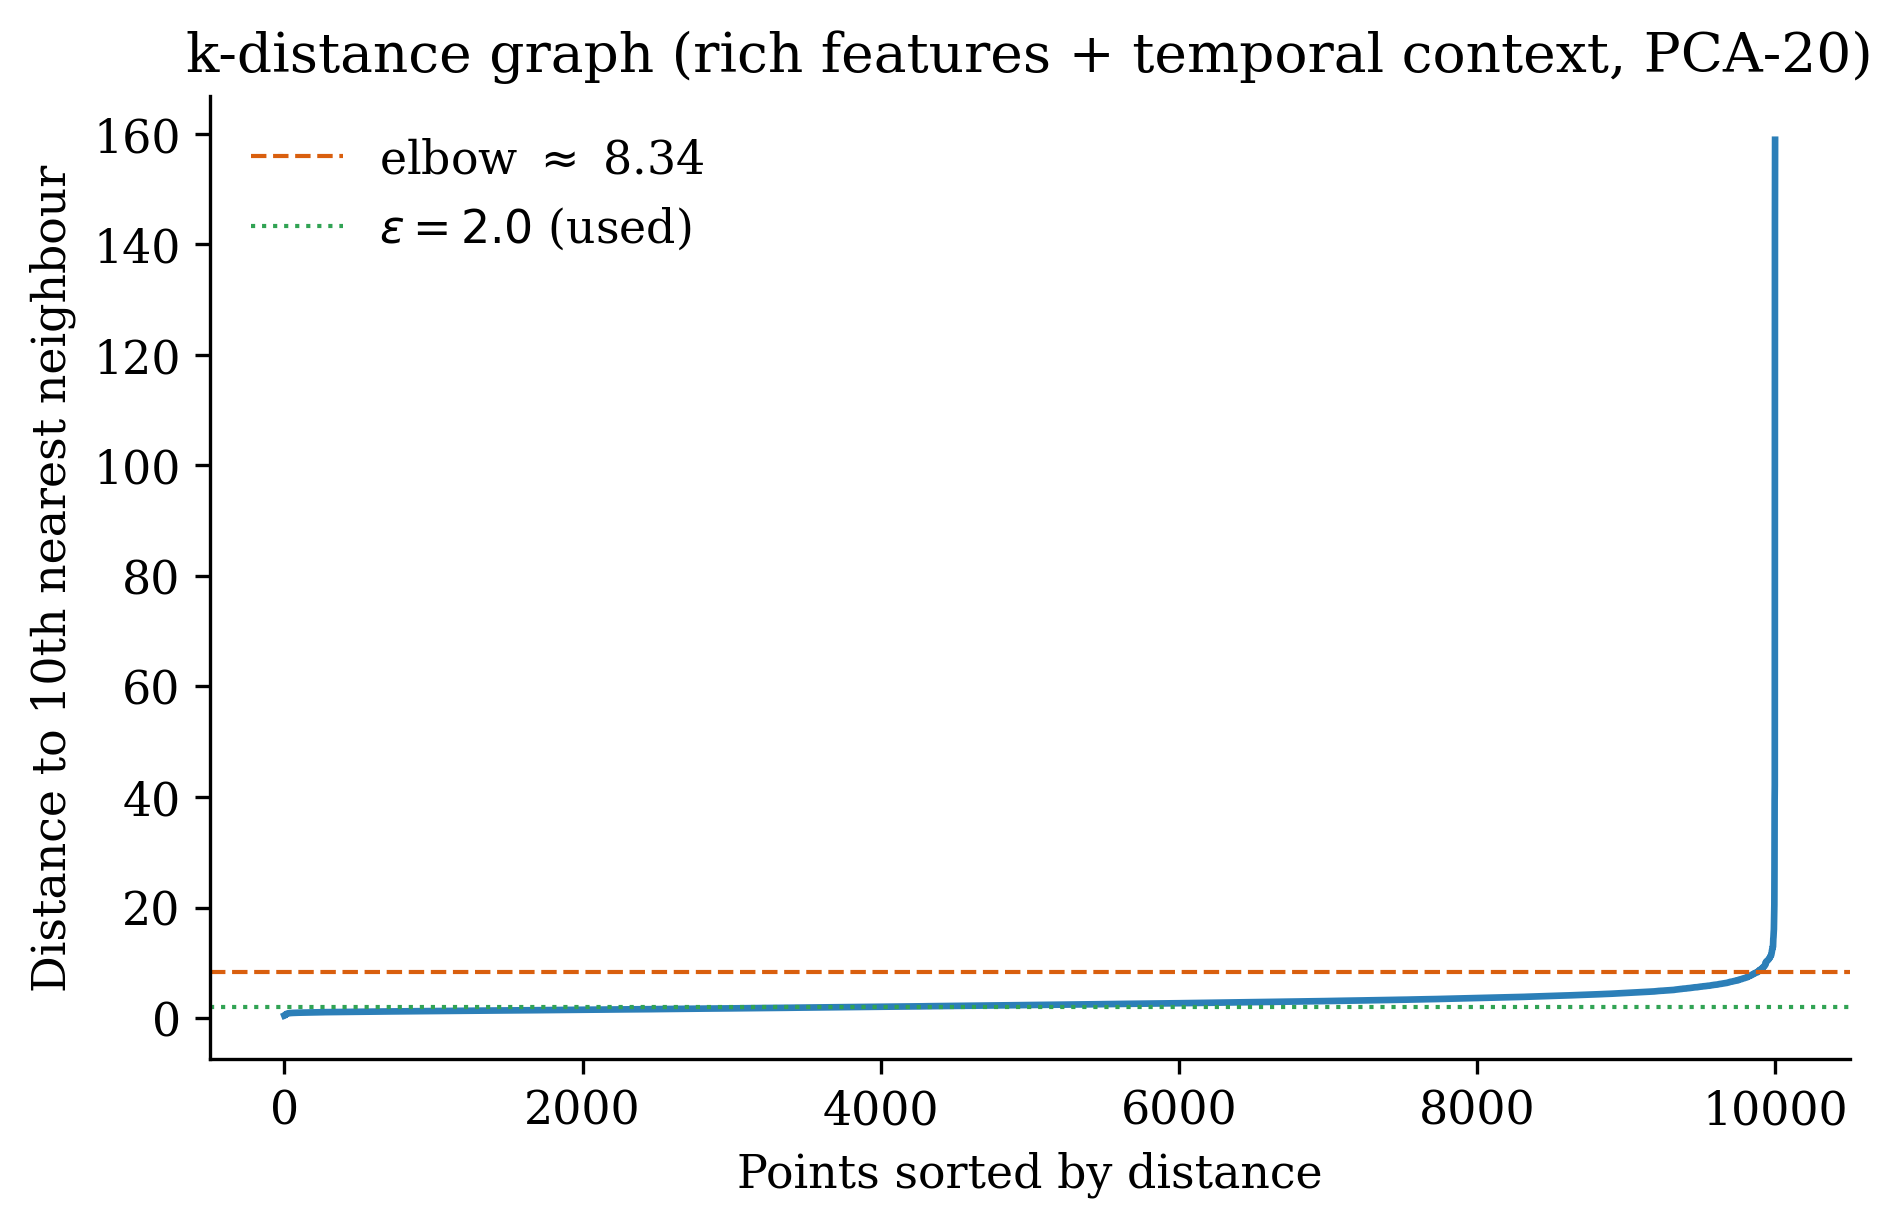
\includegraphics[width=0.6\linewidth]{figures/report/fig_kdistance_rich.png}
\caption{\textbf{$k$-distance graph for the rich-feature space} (39 spectral
features with temporal context, reduced by PCA to 20 dimensions). The natural
elbow lies well above $\varepsilon=2.0$, the radius used for five-cluster recovery;
the chosen radius was guided by clustering stability rather than the elbow alone,
illustrating a known limitation of unsupervised radius selection.}
\label{fig:kdist}
\end{figure}

% =====================================================================
\section{Results}
% =====================================================================
\subsection{The HRV baseline establishes the problem}
The initial ECG/HRV baseline recovered essentially no stage structure: across
algorithms, ARI, AMI and NMI all lay near $0.03$ (Figure~\ref{fig:baseline}a), and
the corresponding projection shows the five stages thoroughly intermixed
(Figure~\ref{fig:baseline}b). This is consistent with the sleep literature:
autonomic HRV captures broad sleep/wake and some REM/NREM differences but is
insufficient for five-stage resolution~\cite{ma2026}. This negative baseline
directly motivated the shift to EEG-centred, richer representations that forms the
remainder of the project.

\begin{figure}[t]
\centering
\begin{subfigure}{0.5\textwidth}
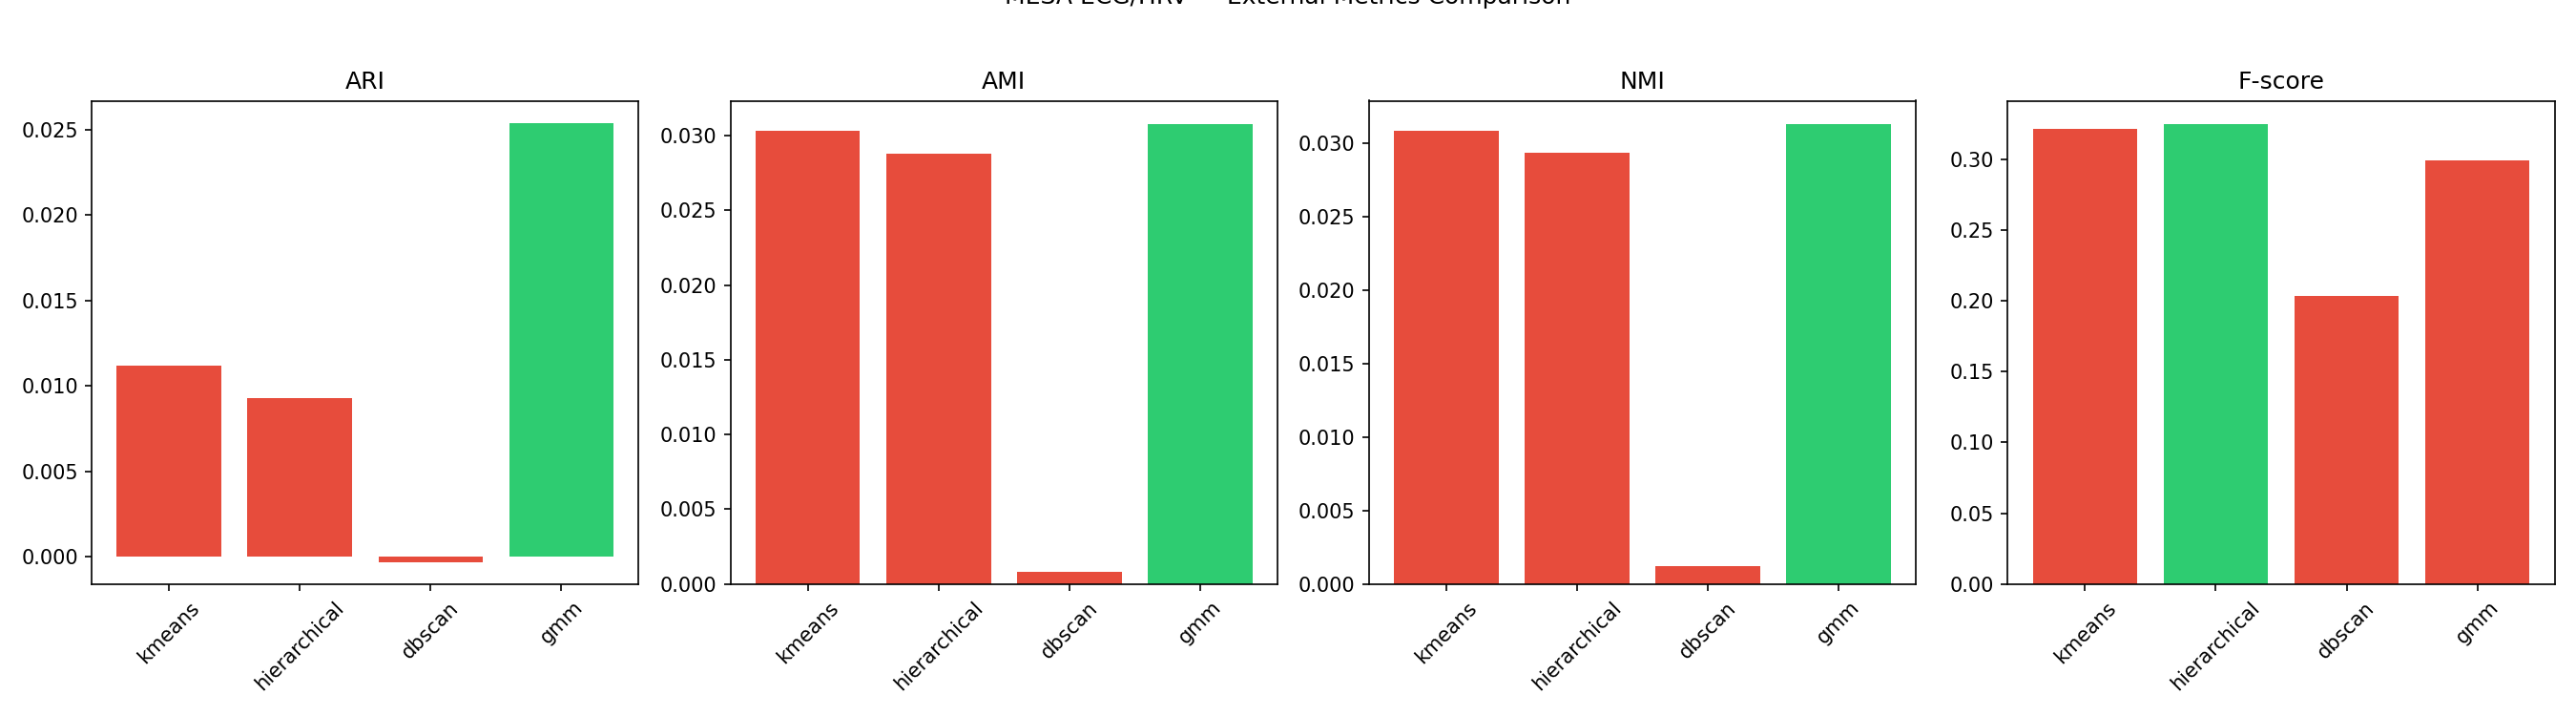
\includegraphics[width=\linewidth]{figures/github/mesa_external_metrics.png}
\caption{}
\end{subfigure}\hfill
\begin{subfigure}{0.47\textwidth}
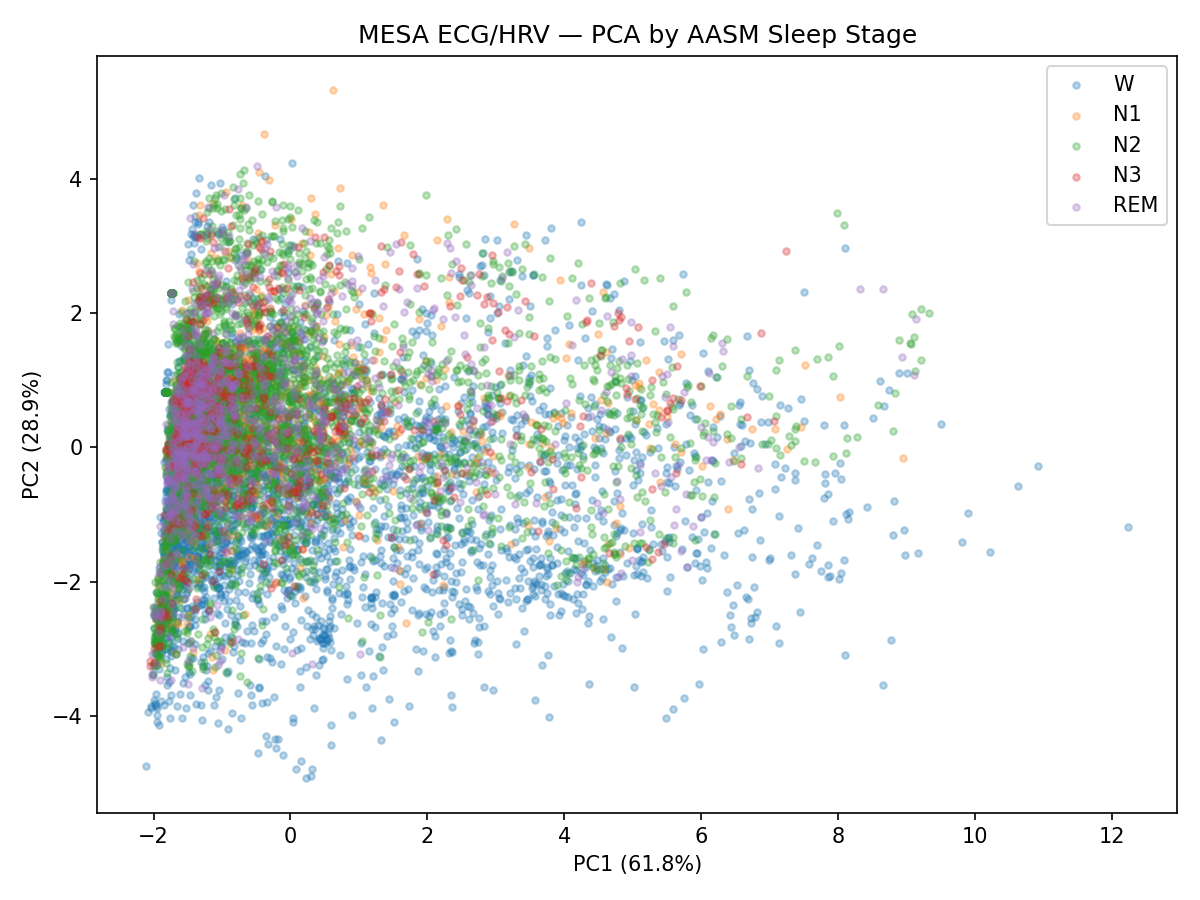
\includegraphics[width=\linewidth]{figures/github/mesa_pca_ground_truth.png}
\caption{}
\end{subfigure}
\caption{\textbf{The ECG/HRV baseline recovers almost no stage structure.}
(a) External agreement metrics across four algorithms are all near zero
(ARI $\approx 0.01$--$0.025$). (b) PCA of HRV features coloured by expert stage:
the five stages overlap almost completely, motivating an EEG-centred approach.}
\label{fig:baseline}
\end{figure}

\subsection{Representation, not algorithm, is the dominant factor}
Moving to EEG and enriching the feature set produced the central result of the
project. Replacing 15 band-power features with the 39 rich spectral features raised
fully unsupervised agreement from $\text{ARI}=0.21$ to $0.28$ and accuracy from
\SI{57.7}{\percent} to \SI{61.7}{\percent} (Figure~\ref{fig:contrib}a). The
cumulative contribution of each component (Figure~\ref{fig:contrib}b) shows richer
features and temporal context each adding roughly $0.07$ ARI over a plain GMM
baseline. The figure also makes plain a result that may at first surprise the
reader: the single step of adding \SI{10}{\percent} of labels contributes more
($\approx 0.22$ ARI) than all of the unsupervised improvements combined,
underscoring how much of the remaining structure is unlocked by even a small
amount of supervision; we return to this in Section~\ref{sec:semisup}. Notably, rich EEG features alone outperformed rich EEG combined with EMG,
SpO\textsubscript{2} and respiration: once the EEG representation is sufficiently
expressive, the additional modalities are largely redundant for coarse stage
structure, reinforcing the primacy of EEG in sleep staging.

\begin{figure}[t]
\centering
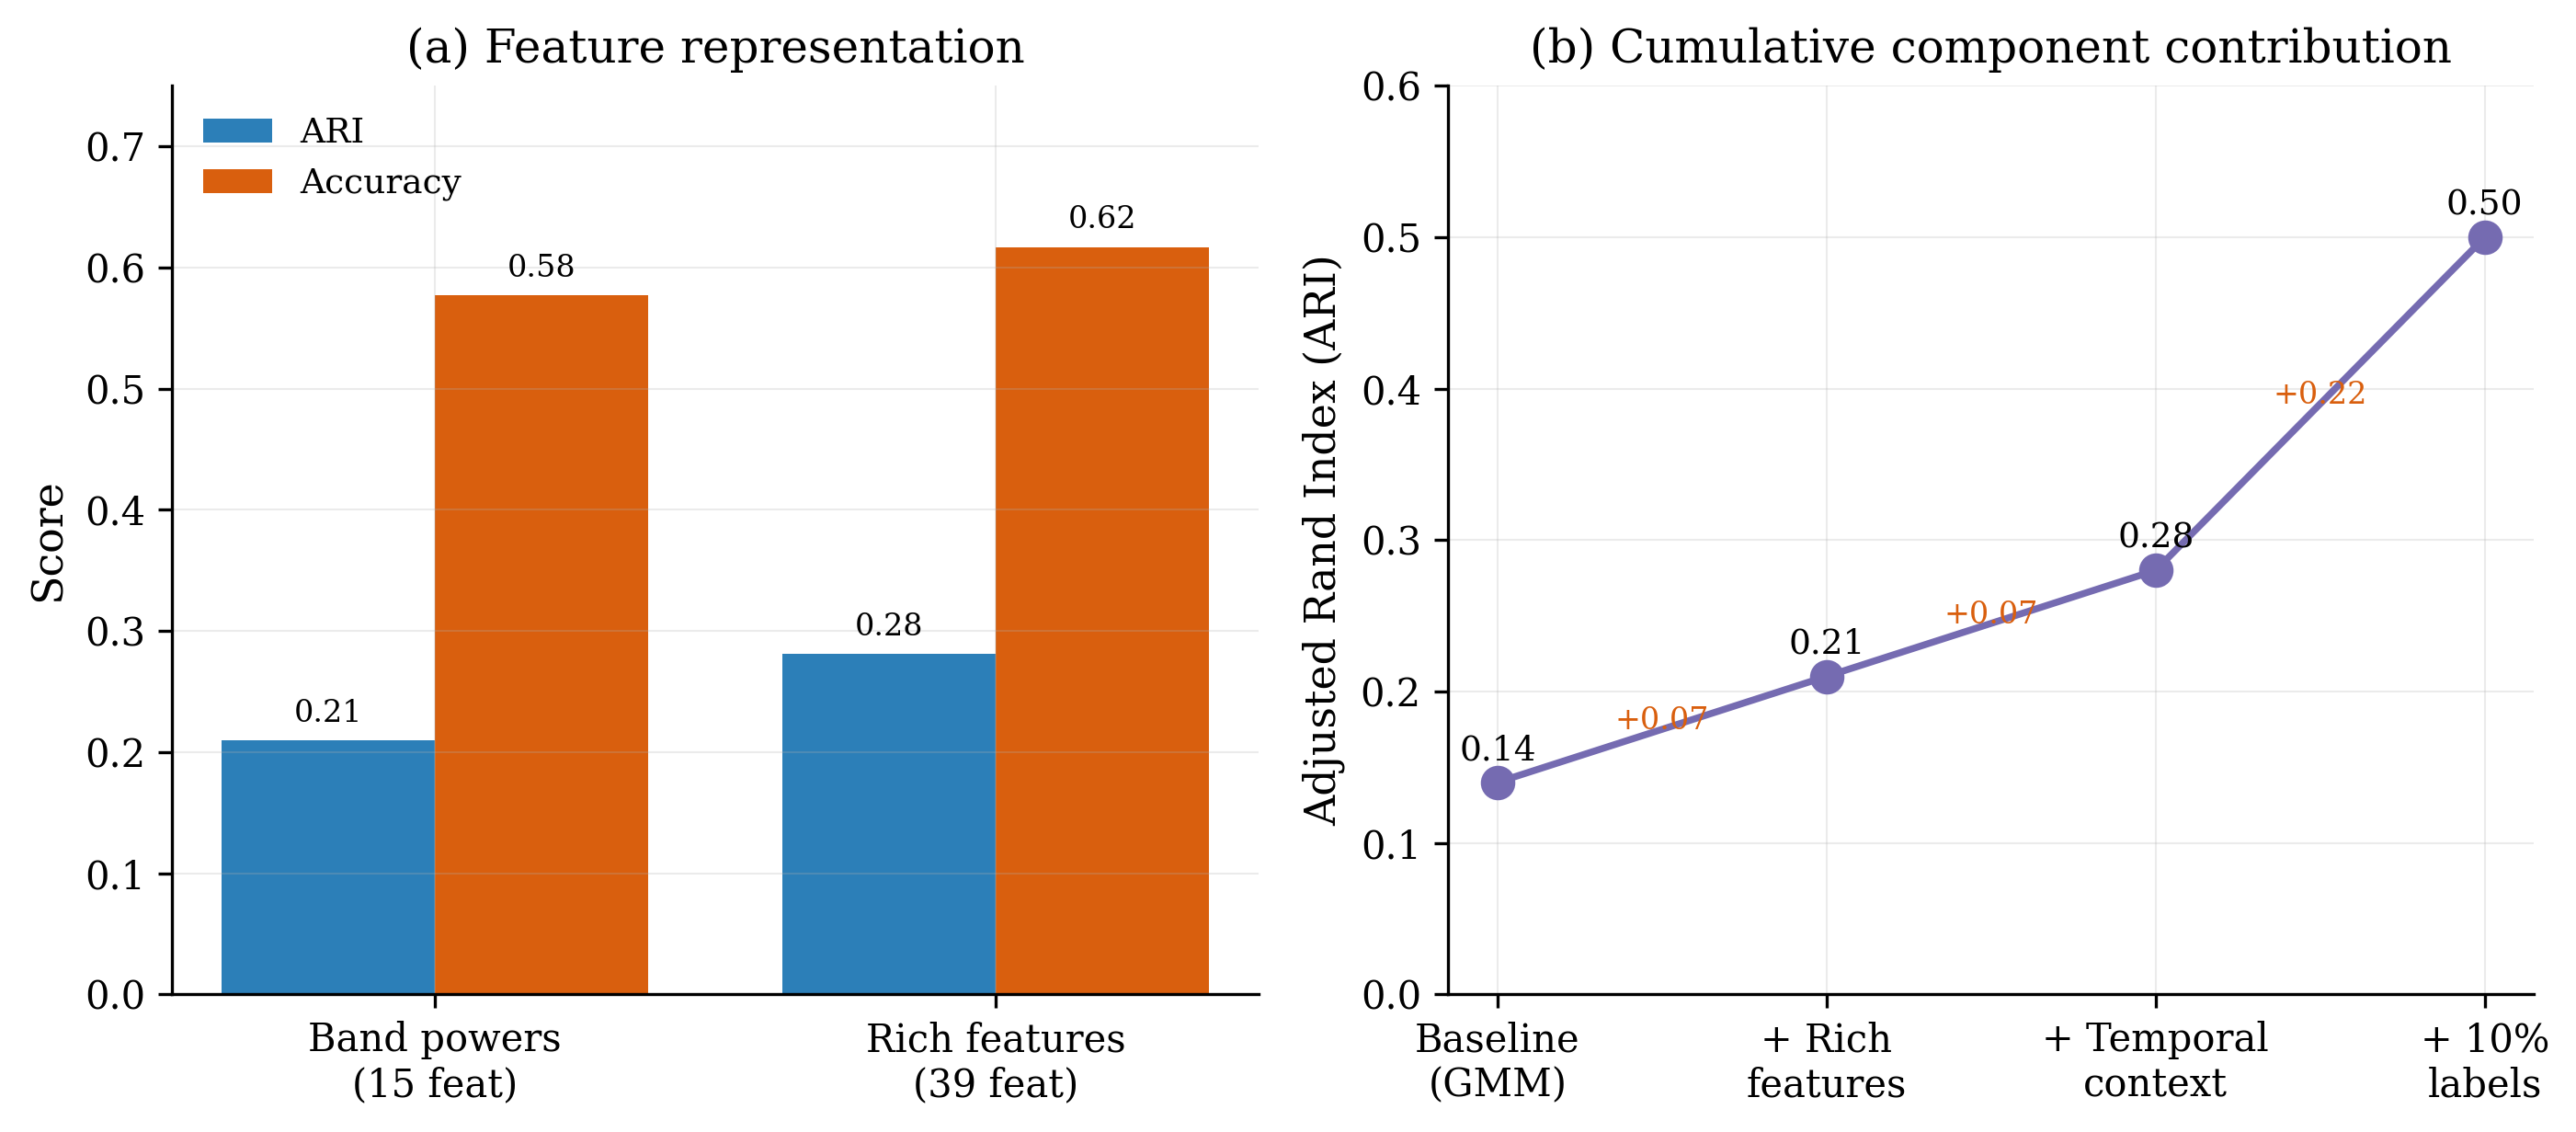
\includegraphics[width=\linewidth]{figures/report/fig2_feature_contributions.png}
\caption{\textbf{Feature representation drives unsupervised performance.}
(a) Rich 39-dimensional spectral features outperform 15 band-power features on both
ARI and accuracy. (b) Cumulative contribution to ARI: richer features and temporal
context each add about $0.07$; a \SI{10}{\percent} labelling budget adds a further
$0.22$.}
\label{fig:contrib}
\end{figure}

\subsection{Which algorithm wins, and why}
Algorithm choice mattered in an interpretable way. Across configurations, GMM and
DBSCAN consistently outperformed $k$-means. This follows from the geometry of the
problem: sleep stages form groups of unequal size and non-spherical shape,
violating the equal-variance, spherical assumptions of $k$-means, whereas GMM
admits full covariances and DBSCAN admits arbitrary cluster shapes and unequal
densities. The best unsupervised configuration (rich features, temporal context,
PCA, DBSCAN at $\varepsilon=2.0$) reached $\text{ARI}=0.28$--$0.32$ and up to
\SI{64.7}{\percent} accuracy ($\kappa=0.43$). A random baseline yielded
$\text{ARI}=0.000\pm0.0001$, confirming that these values reflect genuine structure
rather than chance, and that an ARI of $0.28$ is far from trivial on a five-way,
heavily imbalanced task. The two unsupervised methods therefore serve different
purposes and we recommend them accordingly: DBSCAN maximises overall agreement
(ARI) and is preferable when the goal is faithful recovery of the dominant
structure, whereas the per-subject HMM (Section~\ref{sec:temporal}) maximises
balanced accuracy and is preferable when recovery of the clinically important
minority stages matters more than aggregate agreement.

\begin{table}[t]
\centering
\small
\caption{\textbf{Summary of agreement with expert AASM labels along the supervision
ladder.} Unsupervised and semi-supervised rows are the principal results; the
supervised row is an upper-bound reference only. Semi-supervised subject-level rows
report mean $\pm$ standard deviation across five folds. ARI, adjusted Rand index;
NMI, normalised mutual information; Bal.\ Acc., balanced accuracy.}
\label{tab:main}
\begin{tabular}{llccccc}
\toprule
Regime & Method (labels) & ARI & NMI & Accuracy & Bal.\ Acc. & $\kappa$ \\
\midrule
Baseline      & Random assignment        & 0.000 & 0.001 & 20.0\% & 20.0\% & 0.000 \\
Unsupervised  & HRV + GMM (ECG only)     & 0.025 & 0.031 & --     & --     & --    \\
Unsupervised  & Band-power EEG + DBSCAN  & 0.210 & 0.184 & 57.7\% & 30.6\% & 0.333 \\
Unsupervised  & Rich EEG + DBSCAN        & 0.281 & 0.233 & 61.7\% & 32.8\% & 0.395 \\
Unsupervised  & Rich EEG + per-subj.\ HMM& 0.198 & 0.270 & 45.3\% & 48.1\% & 0.309 \\
Semi-sup.\    & Self-training (10\%)     & 0.500 & --    & 74.3\% & 54.8\% & 0.606 \\
Semi-sup.\    & Label spread.\ (10\%, subj-CV) & $0.38{\pm}0.04$ & -- & $66.3{\pm}2.3\%$ & 52.4\% & $0.51{\pm}0.03$ \\
\textit{(ref.)} & \textit{Supervised RF (subj-CV)} & $0.56{\pm}0.07$ & -- & $77.1{\pm}3.7\%$ & 59.0\% & $0.65{\pm}0.05$ \\
\bottomrule
\end{tabular}
\end{table}

\subsection{Temporal structure is the key unsupervised gain}
\label{sec:temporal}
Augmenting features with temporal context improved unsupervised ARI from $0.14$ to
$0.21$, the largest purely unsupervised gain obtained. We distinguish this
\emph{temporal proximity} effect (adjacent epochs tend to share a stage) from an
earlier experiment using power-spectral shape similarity between epochs, which did
not exceed the band-power baseline; the benefit therefore arises from temporal
adjacency, not signal-shape resemblance. Consistent with this, a per-subject
Gaussian HMM that models stage-transition dynamics achieved the best balanced
accuracy of any unsupervised method (\SI{48.1}{\percent}), recovering the minority
stages markedly better than density clustering despite a lower overall ARI, because
it captures the sequential structure of sleep rather than treating epochs
independently.

\subsection{Per-stage structure}
Aggregating over five cross-validation folds, the recovered stages form a clear
hierarchy (Figure~\ref{fig:perstage}a): REM ($F_1=0.80$) and N1 ($F_1=0.68$) are
recovered best, N2 ($F_1=0.58$) and N3 ($F_1=0.40$) moderately, and Wake
($F_1=0.14$) poorly, with Wake epochs dispersed across other clusters. The
direction of this dispersal is itself informative: the largest share of misassigned
Wake epochs (around \SI{40}{\percent}) falls into N1, with smaller fractions into
REM and N3. This is physiologically sensible, since Wake and N1 are adjacent
light-sleep states that share substantial spectral overlap (attenuated alpha,
low-amplitude mixed-frequency activity), and it is precisely the Wake/N1 boundary
where human inter-rater agreement is also weakest.

\begin{table}[t]
\centering
\small
\caption{\textbf{Per-stage performance} of semi-supervised label spreading
(\SI{10}{\percent} labels), pooled over five subject-level folds. Support is the
number of expert-labelled epochs in the pooled held-out sets.}
\label{tab:perstage}
\begin{tabular}{lcccc}
\toprule
Stage & Precision & Recall & $F_1$ & Support \\
\midrule
REM & 0.816 & 0.788 & \textbf{0.802} & 4333 \\
N1  & 0.655 & 0.711 & \textbf{0.682} & 3314 \\
N2  & 0.549 & 0.603 & 0.575 & 643 \\
N3  & 0.391 & 0.404 & 0.398 & 947 \\
W   & 0.172 & 0.121 & \textbf{0.142} & 763 \\
\bottomrule
\end{tabular}
\end{table} The
embedding (Figure~\ref{fig:perstage}b) shows why the aggregate ARI is bounded: the
discovered clusters capture real structure but overlap substantially with
neighbouring stages, mirroring the genuine physiological ambiguity that also limits
human inter-rater agreement.

\begin{figure}[t]
\centering
\begin{subfigure}{0.46\textwidth}
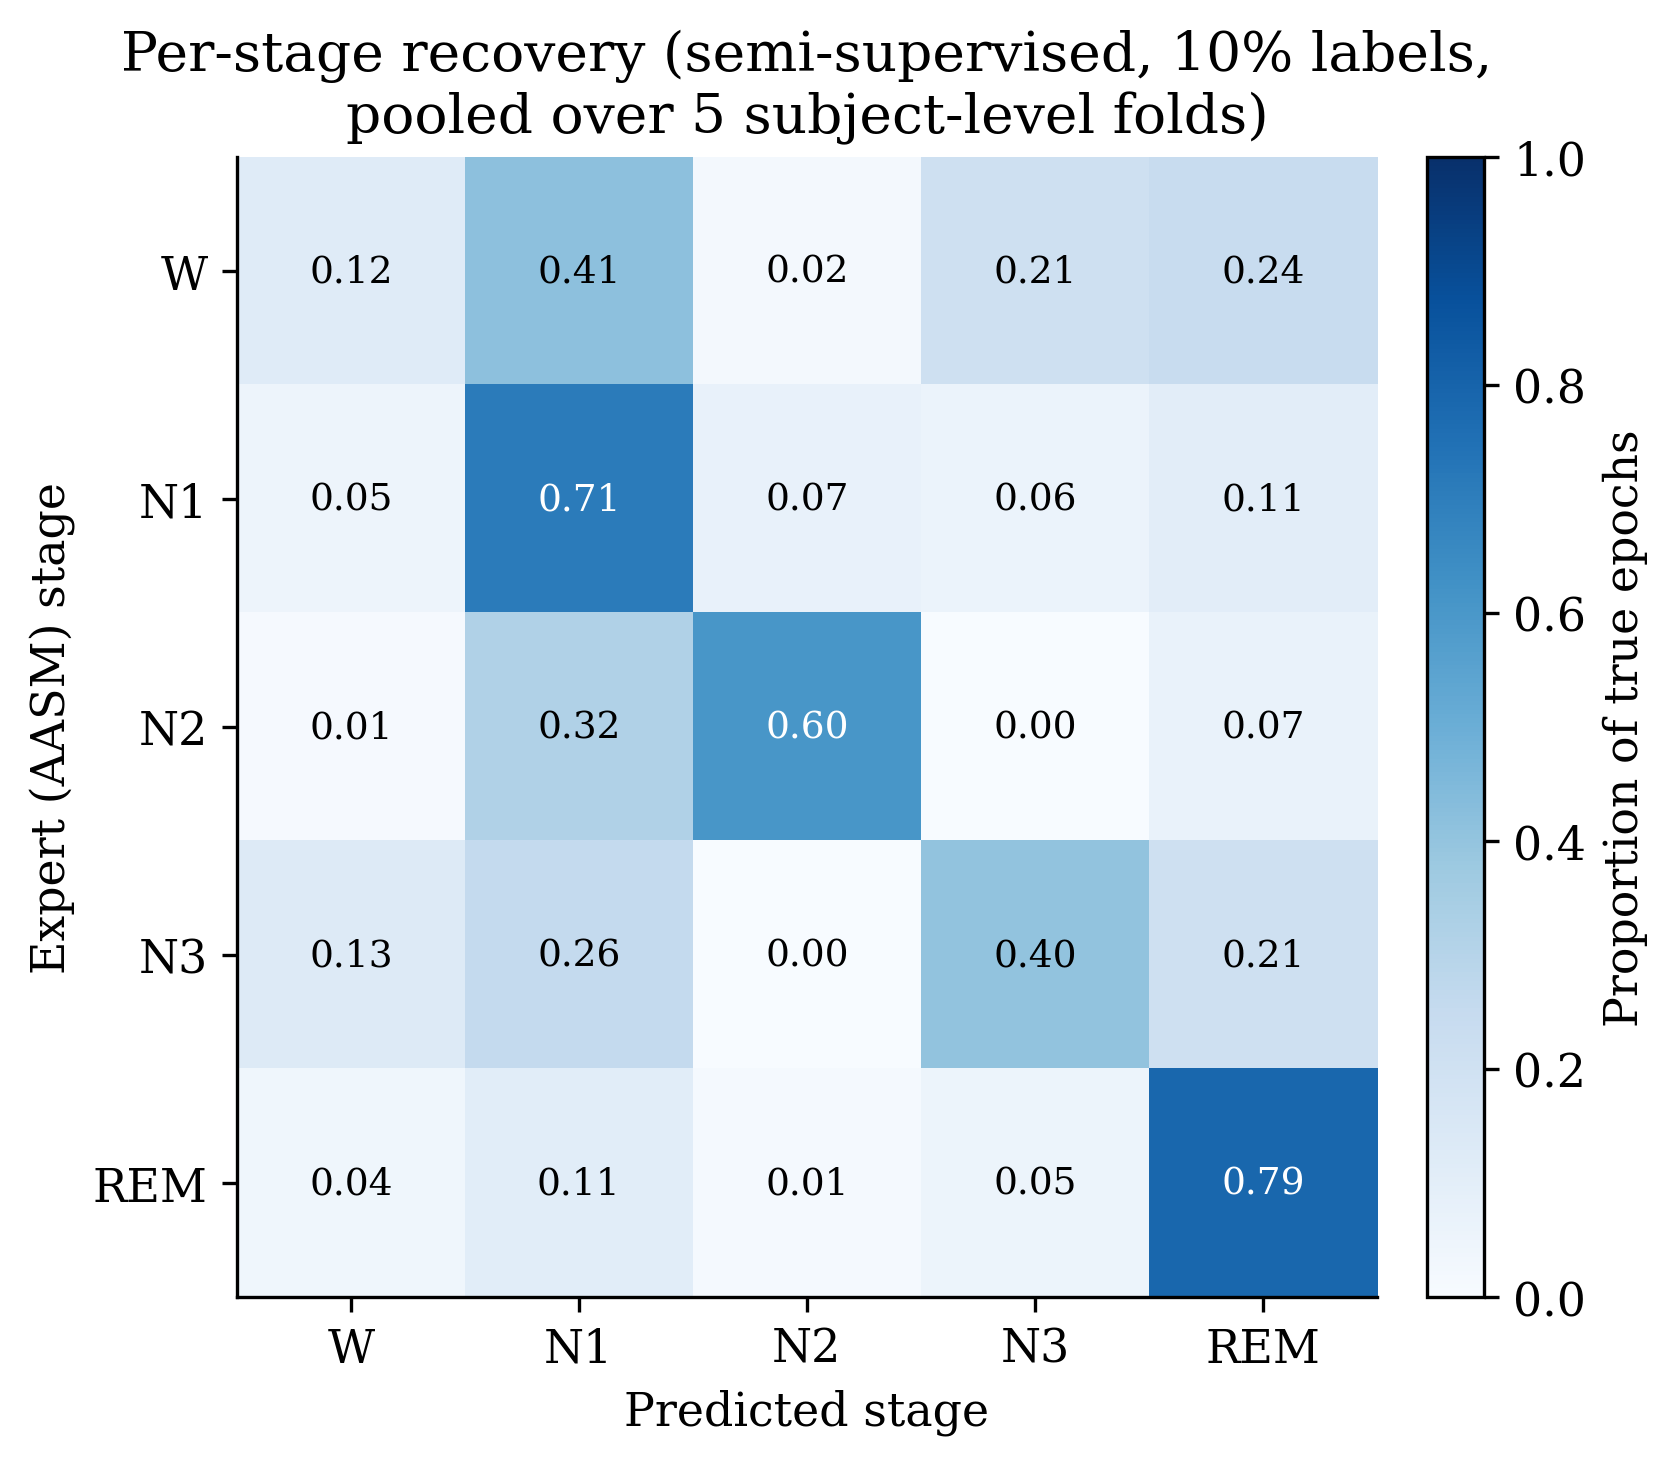
\includegraphics[width=\linewidth]{figures/report/fig4_per_stage_confusion.png}
\caption{}
\end{subfigure}\hfill
\begin{subfigure}{0.50\textwidth}
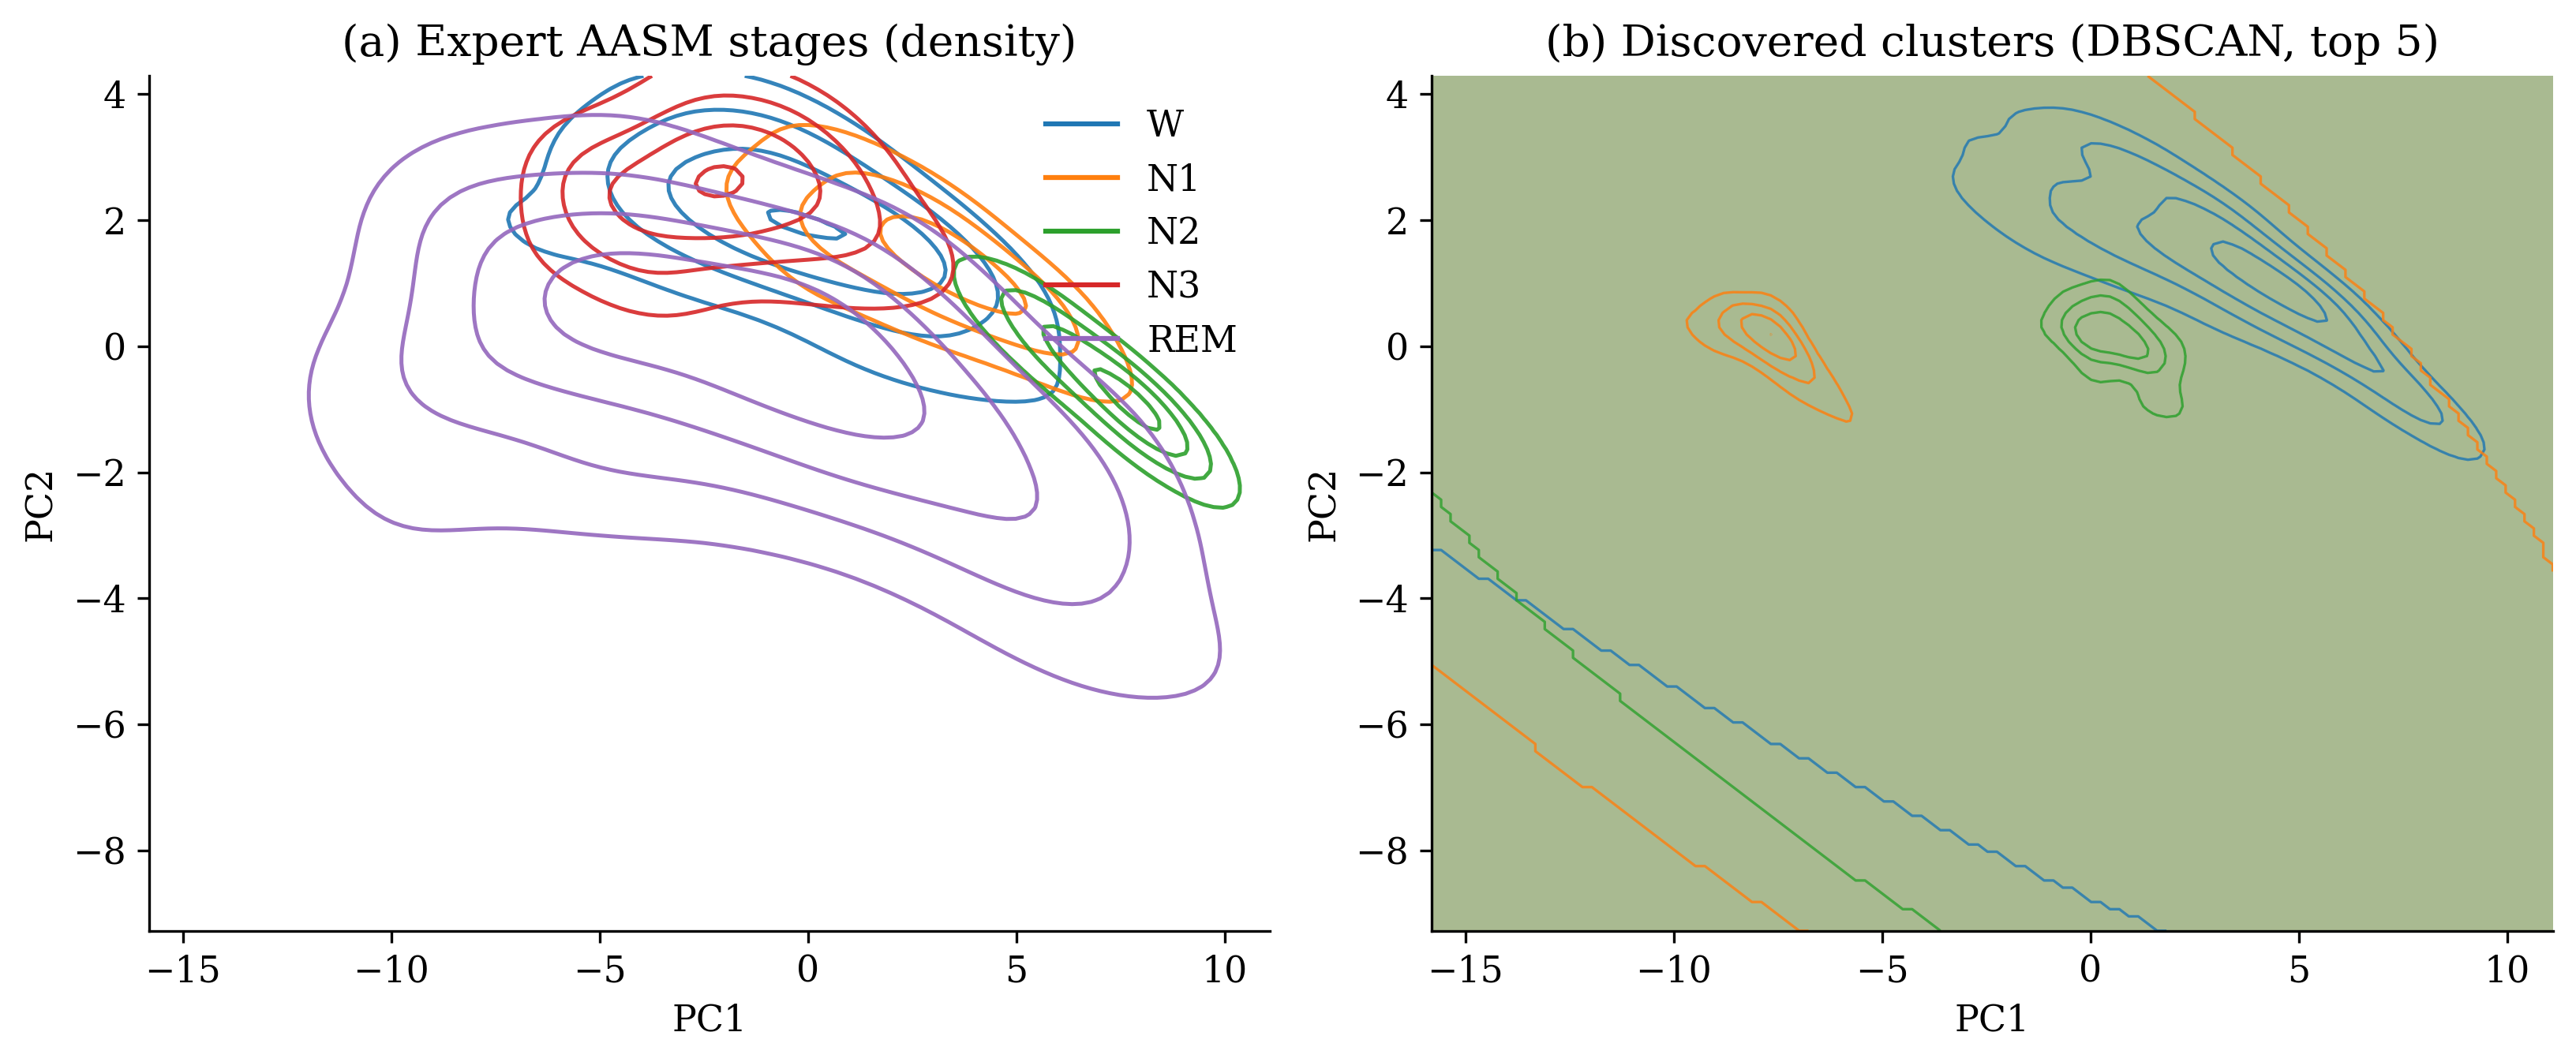
\includegraphics[width=\linewidth]{figures/report/fig6_pca_embedding.png}
\caption{}
\end{subfigure}
\caption{\textbf{Per-stage recovery and embedding structure.}
(a) Row-normalised confusion matrix (pooled over five subject-level folds): REM and
N1 recover well, Wake poorly. (b) PCA density contours of expert stages (left) and
discovered clusters (right): substantial but incomplete overlap bounds the
achievable agreement.}
\label{fig:perstage}
\end{figure}

\subsection{A small labelling budget is highly cost-effective}
\label{sec:semisup}
Although the project is primarily unsupervised, we quantified how performance
improves when a small fraction of labels is available, reflecting the realistic
clinical setting of abundant unlabelled data with limited expert scoring. On
held-out epochs, self-training with \SI{10}{\percent} of labels reached
$\text{ARI}=0.50$ and \SI{74.3}{\percent} accuracy ($\kappa=0.61$). Under the
stricter, leakage-free subject-level cross-validation, label spreading with
\SI{10}{\percent} of labels generalised to unseen subjects at
$\text{ARI}=0.38\pm0.04$ and $66.3\pm2.3\%$ accuracy, with low fold-to-fold
variance (Figure~\ref{fig:ladder}). The gap between these two \SI{10}{\percent}
figures ($74.3\%$ versus $66.3\%$) reflects two compounding differences rather than
inconsistency: they use different methods (self-training versus label spreading)
and, more importantly, different validation schemes, since subject-level
cross-validation forbids same-subject leakage and therefore yields a stricter,
more realistic estimate of generalisation to new individuals. For reference only, a fully supervised random
forest bounds achievable agreement at $\text{ARI}=0.56\pm0.07$ and $77.1\pm3.7\%$
under the same protocol. A \SI{10}{\percent} labelling budget thus closes roughly
half of the gap between the unsupervised result and the supervised ceiling.

\begin{figure}[t]
\centering
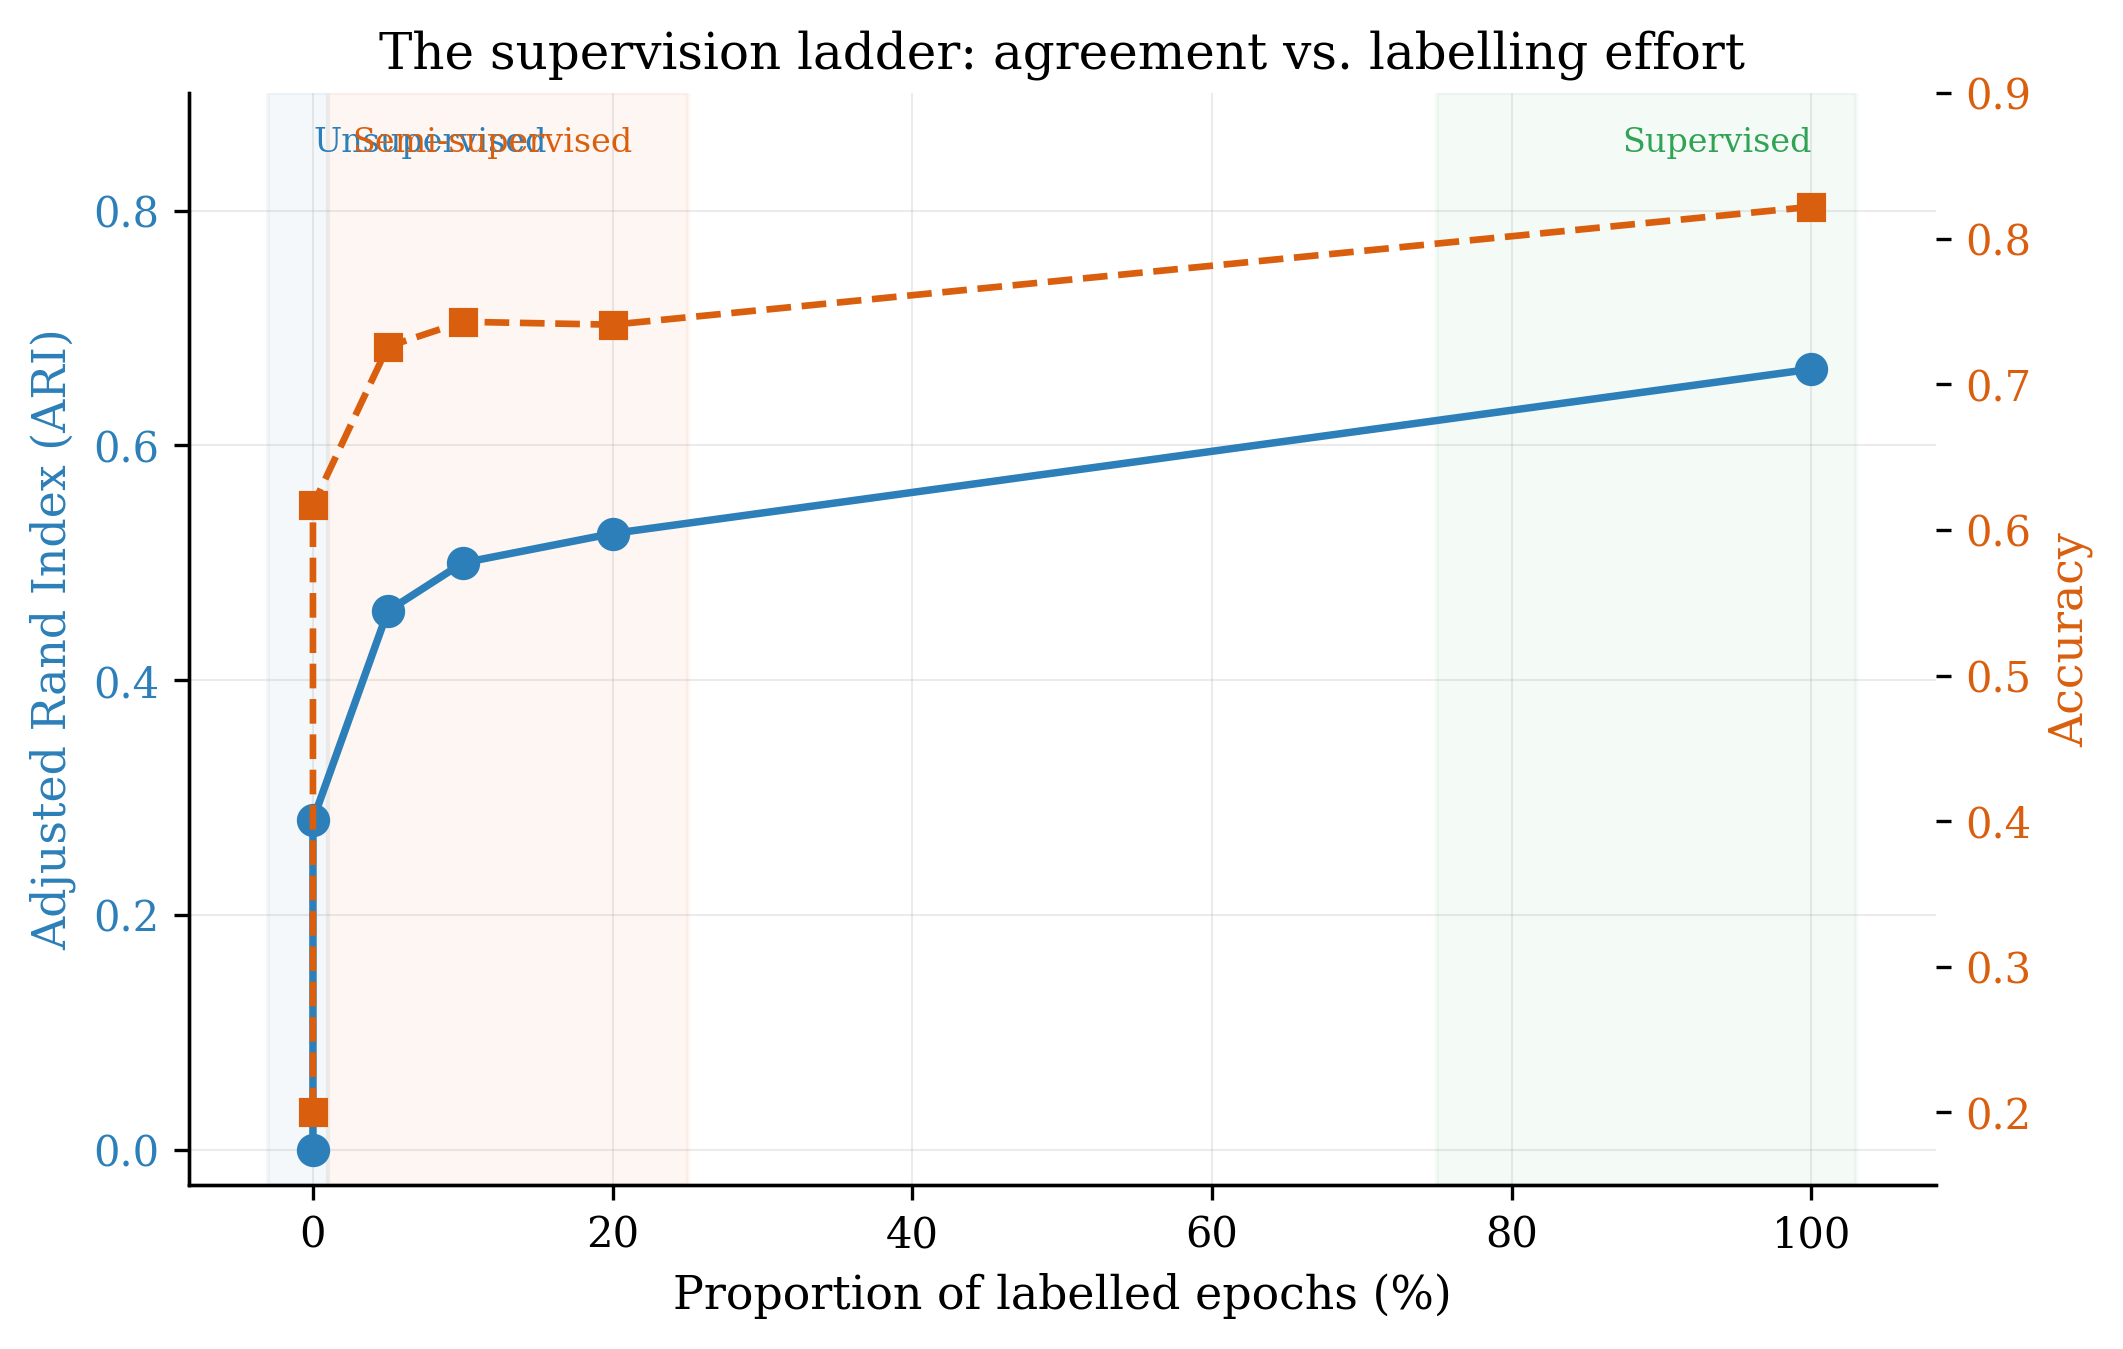
\includegraphics[width=0.84\linewidth]{figures/report/fig1_supervision_ladder.png}
\caption{\textbf{Performance as a function of labelling effort.} ARI (left axis)
and accuracy (right axis) from a random baseline through the fully unsupervised
result to small-budget semi-supervised learning and a fully supervised upper bound.
The steepest gains occur in the first \SI{10}{\percent} of labels.}
\label{fig:ladder}
\end{figure}

\subsection{Deep learning and consensus clustering underperform}
Contrary to the expectation that learned representations would dominate, every deep
approach underperformed the classical pipeline (Figure~\ref{fig:deep}). A feature
autoencoder reached $\text{ARI}=0.14$, Improved Deep Embedded Clustering $0.13$,
and a 1D convolutional autoencoder trained on raw EEG waveforms only $0.02$; the
latter's reconstruction loss barely improved (from $0.68$ to $0.63$), indicating it
captured low-level signal statistics rather than stage-relevant structure.
Consensus clustering, which combines many base partitions through a co-association
matrix, reached only $\text{ARI}=0.07$ because averaging a strong DBSCAN partition
with many weaker base clusterings diluted rather than reinforced it. The classical
pipeline remained the best unsupervised method throughout.

\begin{figure}[t]
\centering
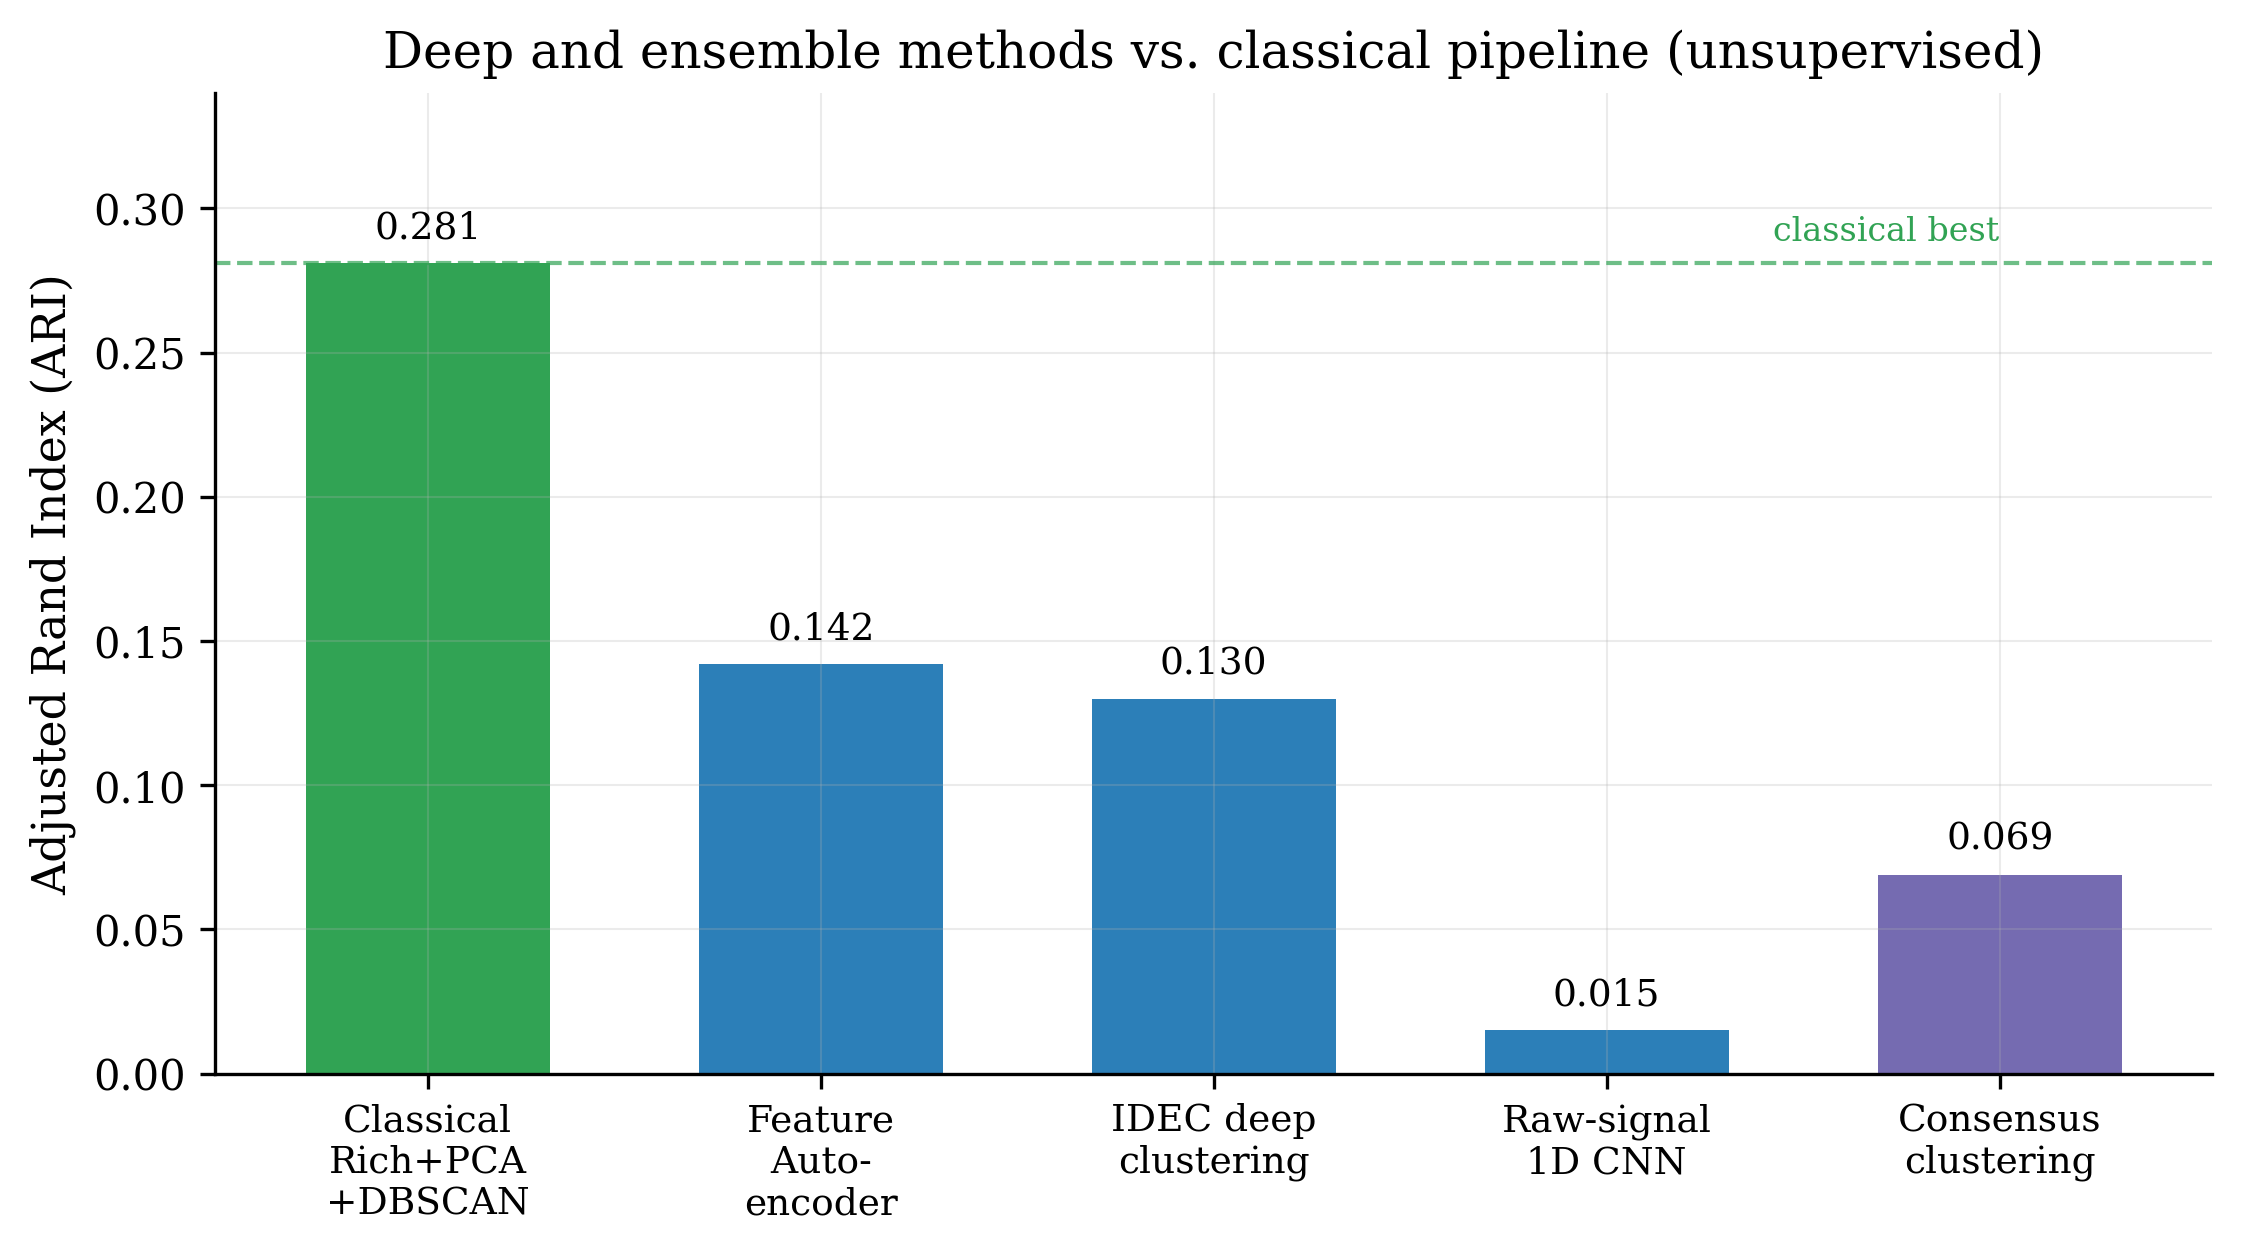
\includegraphics[width=0.8\linewidth]{figures/report/fig3_deep_vs_classical.png}
\caption{\textbf{Deep and ensemble methods do not beat the classical pipeline.}
On engineered features at this dataset scale, feature autoencoders, deep embedded
clustering, raw-waveform CNNs and consensus clustering all fall below the classical
rich-features + PCA + DBSCAN result (dashed line).}
\label{fig:deep}
\end{figure}

% =====================================================================
\section{Discussion}
% =====================================================================
\subsection{Interpretation}
Our results give a qualified, data-driven endorsement of the conclusion of Ma et
al.~\cite{ma2026}: the AASM five-stage structure is \emph{partially} recoverable
from unlabelled physiology. With purely unsupervised methods we reach
$\text{ARI}=0.28$ and \SI{61.7}{\percent} accuracy, well above chance but far below
the supervised ceiling, and the per-stage analysis shows that this aggregate masks
a strong gradient: REM and N1 emerge naturally from the signal, whereas Wake does
not.

It is instructive to situate these figures against Ma et al.~\cite{ma2026}
quantitatively. Their fuzzy subspace clustering of 64--136 EEG/EOG/EMG features
identified five clusters as optimal and reported cluster-to-stage correspondence
appreciably higher than our $\text{ARI}=0.28$. The gap is informative rather than
contradictory and follows from three design choices. First, representation: they
used a far richer, multi-modal feature set with explicit per-feature subspace
weighting, whereas we deliberately probed how far a compact, interpretable 39-feature
EEG representation could go. Second, cohort: they evaluated on curated research
databases (MNC and HMC), while MESA is an unselected community cohort carrying the
artefacts, comorbidity and demographic heterogeneity of large-scale epidemiological
data, which depresses absolute agreement. Third, algorithm: subspace weighting
effectively performs soft feature selection that plain density clustering does not.
That a substantially simpler pipeline still recovers a clear five-way gradient
independently corroborates their central claim that the five stages are a genuine,
if imperfect, emergent property of sleep physiology rather than a purely
conventional construct; and our supervised reference ($\text{ARI}=0.56$,
\SI{77}{\percent}) sitting below the $\sim$\SI{80}{\percent} of dedicated supervised
stagers is consistent with the ``expert imitator'' ceiling they describe, since any
label-referenced model is bounded by the reliability of its training labels.

The poor recovery of Wake ($F_1=0.14$), with around \SI{40}{\percent} of Wake
epochs absorbed into N1, is the most clinically consequential failure and merits
specific attention. In MESA, a community cohort, much ``Wake'' is quiet wakefulness
and wake-after-sleep-onset rather than alert eyes-open wake, and quiet wake shares
attenuated-alpha, low-amplitude mixed-frequency activity with N1, so the two are
genuinely adjacent in spectral space. Clinically this matters because the Wake/N1
boundary determines sleep-onset latency and wake-after-sleep-onset, two of the
metrics most used to quantify insomnia and sleep fragmentation; an unsupervised
stager that cannot separate quiet wake from N1 would systematically misestimate
these indices, which is an important caveat for any label-free deployment.

Finally, the temporal-proximity result connects directly to established sleep
physiology. Sleep is organised into roughly 90-minute NREM--REM cycles with strong
stage persistence, and the AASM rules themselves encode temporal continuity through
their transition and arousal criteria. Our finding that a simple neighbour-averaging
window, and more strongly a per-subject HMM, improves recovery, while signal-shape
similarity does not, is the data-driven counterpart of that domain knowledge: the
information added by temporal context is the high self-transition probability of
sleep stages, exactly the structure the HMM transition matrix captures, which
explains why it most improves the persistent minority stages. The success of the
HMM at recovering these stages reinforces that modelling the sequential structure of
sleep, rather than treating epochs independently, is valuable.

\subsection{Why deep learning did not win}
The consistent underperformance of deep methods is, at first glance, surprising
given their dominance in supervised staging, and we attribute it to three factors.
First, scale: with on the order of $10^4$ epochs and CPU training, the data are
insufficient for representation learning to surpass domain-informed features.
Second, objective mismatch: reconstruction-driven autoencoders spend capacity
faithfully rebuilding noisy waveforms, much of which is irrelevant to staging,
whereas spectral features discard that noise by construction. Third, feature
quality: the 39 engineered descriptors already encode the spectral and complexity
information a network would have to rediscover. This mirrors a broader pattern in
physiological machine learning in which, below a data-scale threshold, expert
features remain competitive. We present this as a useful negative result that
delimits when deep learning is warranted for cohorts of this size, rather than as a
failure.

\subsection{Limitations}
Several limitations temper these conclusions. The analysis uses 100 subjects;
while this yields a large epoch count, subject-level diversity is limited, and the
subject-level cross-validation, though leakage-free, still draws from a single
cohort. Performance is bounded by the genuine overlap of stages in feature space
(Figure~\ref{fig:perstage}b), a property of the physiology rather than of the
algorithm. A methodological caveat concerns the DBSCAN radius: although it was not
tuned against labels, the value used for five-cluster recovery lies below the
$k$-distance elbow (Figure~\ref{fig:kdist}) and was selected for clustering
stability, so the recovery is somewhat sensitive to this choice; a fully
label-free criterion for selecting the radius best suited to a target number of
clusters remains an open problem. The SpO\textsubscript{2} channel exhibited artefacts (physiologically implausible
saturation values and dropouts) that limited its contribution; because the rich
EEG representation already accounted for the coarse stage structure and
SpO\textsubscript{2} added little on top of it, we did not pursue dedicated
artefact correction for this channel. A more careful treatment of the oximetry
signal, which is clinically central to sleep-disordered breathing, is a reasonable
avenue for extracting additional value from this modality. The deep-learning experiments were constrained to CPU training and,
for the raw-waveform model, a single EEG channel, so they do not exclude the
possibility that larger multi-channel networks trained on far more data would
perform better. Finally, like all label-referenced evaluations, our metrics inherit
the subjectivity of the AASM annotations; the poor recovery of Wake may partly
reflect genuine ambiguity in the reference labels rather than a failure of
clustering.

\subsection{Future work}
Three directions follow naturally. First, scaling to several hundred subjects would
test whether deep representation learning crosses the data-scale threshold at which
it begins to outperform engineered features, and would tighten the confidence
intervals. Second, incorporating \emph{pretrained} sleep foundation-model
embeddings, as opposed to from-scratch autoencoders, is the most promising route to
richer unlabelled representations and was identified by our supervisor as the
highest-leverage next step. Third, sleep-specific features targeting the weakest
stages, including sleep-spindle and K-complex detection for N2 and N3 and refined
EOG--EEG coupling for REM, would directly address the per-stage deficiencies
identified here.

% =====================================================================
\section{Conclusion}
% =====================================================================
We studied the unsupervised recovery of AASM sleep stages from MESA
polysomnography. Beginning from an HRV baseline that recovered no stage structure,
we showed that feature representation, rather than the choice of clustering
algorithm, is the dominant factor: rich spectral EEG features with temporal context
and density-based clustering recovered the five stages at $\text{ARI}=0.28$ and
\SI{61.7}{\percent} accuracy, well above a calibrated random baseline. Gaussian
mixture and density methods outperformed $k$-means for principled geometric
reasons, temporal proximity provided the largest unsupervised gain, and a
per-subject hidden Markov model best recovered the minority stages. A modest
\SI{10}{\percent} labelling budget proved highly cost-effective, reaching
\SI{66}{\percent} accuracy on unseen subjects, while deep representation learning
and consensus clustering did not improve on engineered features at this scale.
These results offer qualified, data-driven support for the five-stage paradigm and
identify representation and temporal structure as the highest-leverage ingredients
for label-free sleep staging.

% =====================================================================
\section*{Data and Code Availability}
% =====================================================================
\small
All analysis code, result tables and figures are available at
\url{https://github.com/namankansal2022/SCDL3991-Sleep-Phenotyping}. The MESA Sleep
Study is available via the National Sleep Research Resource at
\url{https://sleepdata.org/datasets/mesa}.

% =====================================================================
\begin{thebibliography}{9}
\small
\bibitem{ma2026}
Ma Y, Li C, Xu Y, Tan X, Yu X, Zhan CA.
Unsupervised clustering of extensive physiological features substantiates
five-stage sleep staging paradigm.
\emph{Sleep}. 2026;49(2):zsaf284.

\bibitem{levy2023}
Levy J, \'Alvarez D, Del Campo F, Behar JA.
Deep learning for obstructive sleep apnea diagnosis based on single channel
oximetry.
\emph{Nature Communications}. 2023;14:4881.

\bibitem{zhang2018}
Zhang GQ, Cui L, Mueller R, et al.
The National Sleep Research Resource: towards a sleep data commons.
\emph{Journal of the American Medical Informatics Association}.
2018;25(10):1351--1358.

\bibitem{chen2015}
Chen X, Wang R, Zee P, et al.
Racial/ethnic differences in sleep disturbances: the Multi-Ethnic Study of
Atherosclerosis (MESA).
\emph{Sleep}. 2015;38(6):877--888.

\bibitem{guenoune}
Güne\c{s} S, Polat K, Yosunkaya \c{S}.
Efficient sleep stage recognition system based on EEG signal using $k$-means
clustering based feature weighting.
\emph{Expert Systems with Applications}. 2010;37(12):7922--7928.

\bibitem{boudreau}
Boudreau P, Yeh WH, Dumont GA, Boivin DB.
Circadian variation of heart rate variability across sleep stages.
\emph{Sleep}. 2013;36(12):1919--1928.

\bibitem{aasm}
Berry RB, Brooks R, Gamaldo CE, et al.
The AASM Manual for the Scoring of Sleep and Associated Events.
American Academy of Sleep Medicine; 2012.
\end{thebibliography}

\end{document}
